%%%%%%%%%%%%%%%%%%%%%%%%%%%%%%%%%%%%%%%%%%%%%%%%%%%%%%%%%%%%%%%%%%%%%%%%%%%%%%
% Customisable conference poster template with BioMedIA logo and Imperial 
% colour style.
%  
% Adapted from Kevin Keraudren's template from the internal BioMedIA pages
% and from baposter/examples/ECCS2011/poster.tex 
% 
% Author: Christian Baumgartner (c.f.baumgartner@gmail.com)
% Date: 11. October 2016
%

% add "debug" as option for debugging output
\documentclass[a0paper,portrait]{baposter}

\usepackage{relsize}                  % For \smaller
\usepackage{url}                      % For \url
\usepackage{epstopdf}                 % Included EPS files automatically converted to PDF to
                                      % include  with pdflatex

\usepackage{multicol}                 % multiple columns
\usepackage[superscript,nomove]{cite} % for superscript citing

\usepackage{enumitem}                 % to change leftmargin of bullet lists
\usepackage{booktabs}                 % nicer tables

\usepackage{tikz}                     % To draw background

%%% Global Settings %%%%%%%%%%%%%%%%%%%%%%%%%%%%%%%%%%%%%%%%%%%%%%%%%%%%%%%%%%%

\graphicspath{{figures/}}            % Root directory of the pictures 
\tracingstats=2                      % Enabled LaTeX logging with conditionals

%%% Color Definitions %%%%%%%%%%%%%%%%%%%%%%%%%%%%%%%%%%%%%%%%%%%%%%%%%%%%%%%%%

% Those are the official imperial colours:
\definecolor{Navy}{RGB}{0,33,71}
\definecolor{ImperialBlue}{RGB}{0,62,116}
\definecolor{LightGrey}{RGB}{235,238,238}
\definecolor{CoolGrey}{RGB}{157,157,157}
\definecolor{LightBlue}{RGB}{212,239,252}
\definecolor{Black}{RGB}{0,0,0}
\definecolor{White}{RGB}{255,255,255}

%%%%%%%%%%%%%%%%%%%%%%%%%%%%%%%%%%%%%%%%%%%%%%%%%%%%%%%%%%%%%%%%%%%%%%%%%%%%%%%% 
%%% Utility functions %%%%%%%%%%%%%%%%%%%%%%%%%%%%%%%%%%%%%%%%%%%%%%%%%%%%%%%%%%

%%% Save space in lists. Use this after the opening of the list %%%%%%%%%%%%%%%%
\newcommand{\compresslist}{
  \setlength{\itemsep}{3pt}
  \setlength{\parskip}{2pt}
  \setlength{\parsep}{2pt}

\vspace{-0.75em}

}

\newcommand{\tab}{\hspace{0.5em}}

%%%%%%%%%%%%%%%%%%%%%%%%%%%%%%%%%%%%%%%%%%%%%%%%%%%%%%%%%%%%%%%%%%%%%%%%%%%%%%% 
%%% Document Start %%%%%%%%%%%%%%%%%%%%%%%%%%%%%%%%%%%%%%%%%%%%%%%%%%%%%%%%%%%%
%%%%%%%%%%%%%%%%%%%%%%%%%%%%%%%%%%%%%%%%%%%%%%%%%%%%%%%%%%%%%%%%%%%%%%%%%%%%%%% 

\begin{document}
\typeout{Poster rendering started}

%%% Setting Background Image %%%%%%%%%%%%%%%%%%%%%%%%%%%%%%%%%%%%%%%%%%%%%%%%%%

\background{
  % Change colours of body background and header background if desired
  % you can also use tikz to include a custom picture here
  \begin{tikzpicture}[remember picture,overlay]%
    %the poster background colour
    \fill[fill=LightGrey] (current page.north west) rectangle (current page.south east);
    %the header
    \fill [fill=LightGrey] (current page.north west) rectangle ([yshift=-\headerheight] current page.north east);
  \end{tikzpicture}
}

%%%   General Poster Settings %%%%%%%%%%%%%%%%%%%%%%%%%%%%%%%%%%%%%%%%%%%%%%%%%%%
%%%%%%   Eye Catcher, Title, Authors and University Images %%%%%%%%%%%%%%%%%%%%%%

\begin{poster}{
  grid=false,
  eyecatcher=true, 
  borderColor=White,
  headerColorOne=ImperialBlue,
  headerColorTwo=ImperialBlue,
  headerFontColor=LightGrey,
  boxColorOne=White,
  headershape=roundedright,
  textborder=roundedleft,
  background=user,
  headerborder=none, 
  textborder=none,
  boxshade=plain
}
%%% Eye Cacther %%%%%%%%%%%%%%%%%%%%%%%%%%%%%%%%%%%%%%%%%%%%%%%%%%%%%%%%%%%%%%%
{
  % nothing here
}
%%% Title %%%%%%%%%%%%%%%%%%%%%%%%%%%%%%%%%%%%%%%%%%%%%%%%%%%%%%%%%%%%%%%%%%%%%
{
  {\sf\bf \textcolor{Black}{Real-time Standard Scan Plane Detection\\\vspace{6pt}
  and Localisation in Fetal Ultrasound}}
  \vspace{3pt} % move authors list down a little bit
} 
%%% Authors %%%%%%%%%%%%%%%%%%%%%%%%%%%%%%%%%%%%%%%%%%%%%%%%%%%%%%%%%%%%%%%%%%%
{
  \textcolor{Black}{Christian F. Baumgartner, Konstantinos Kamnitsas, Jacqueline 
  Matthew, Sandra Smith,\\ Bernhard Kainz, Daniel Rueckert} 
}
%%% Logo %%%%%%%%%%%%%%%%%%%%%%%%%%%%%%%%%%%%%%%%%%%%%%%%%%%%%%%%%%%%%%%%%%%%%%
{
  
\includegraphics[width=0.2\textwidth]{logos/biomedia}
}

%%%%%%%%%%%%%%%%%%%%%%%%%%%%%%%%%%%%%%%%%%%%%%%%%%%%%%%%%%%%%%%%%%%%%%%%%%%%%%% 
%%% Boxes Start %%%%%%%%%%%%%%%%%%%%%%%%%%%%%%%%%%%%%%%%%%%%%%%%%%%%%%%%%%%%%%%
%%%%%%%%%%%%%%%%%%%%%%%%%%%%%%%%%%%%%%%%%%%%%%%%%%%%%%%%%%%%%%%%%%%%%%%%%%%%%%% 

%%% Motivation %%%%%%%%%%%%%%%%%%%%%%%%%%%%%%%%%%%%%%%%%%%%%%%%%%%%%%%%%%%%%%%%
\headerbox{Motivation}{name=motivation,column=0,row=0}{

Numerous countries have introduced fetal {\bf screening programmes} 
to improve early detection of fetal abnormalities: 

\begin{itemize}[leftmargin=1.4em]
  \compresslist
  \item This generates a {\bf very high work load }for a limited number 
  of sonographers. 
  \item Detecting abnormalities can be {\bf very challenging} ($\approx 74\%$ 
  detection rate, with large geographic variations).
  \item In developing countries the majority of ultrasound scans are carried 
  out by non-experts\cite{salomon2011practice}.
  \item Computer vision methods can be used to develop tools to assist 
  sonographers with this demanding task and reduce their workload. 
\end{itemize}
\vspace{-5pt}
\emph{Contributions:} According to national guidelines, sonographers need to 
acquire data from fixed standard views to (1) obtain measurements, (2) check for 
abnormalities and (3) document the case. We propose a method to:

\begin{itemize}[leftmargin=1.4em]
  \compresslist
  \item Guide sonographers: automatically and {\bf robustly} detect 12 standard 
  scan planes in {\bf real-time, free hand} 2D ultrasound scans. 
  \item Help inexperienced users: {\bf Retrospectively retrieve} standard views 
  from recorded videos with accuracy approaching that of sonographers. 
  \item {\bf Localise fetal anatomy} in image stream {\bf without supervision}.
\end{itemize}  

}

%%% Overview %%%%%%%%%%%%%%%%%%%%%%%%%%%%%%%%%%%%%%%%%%%%%%%%%%%%%%%%%%%%%%%%%%
\headerbox{Overview}{name=overview,column=1,span=2, row=0}{

\begin{minipage}[c]{\textwidth}
    \centering
    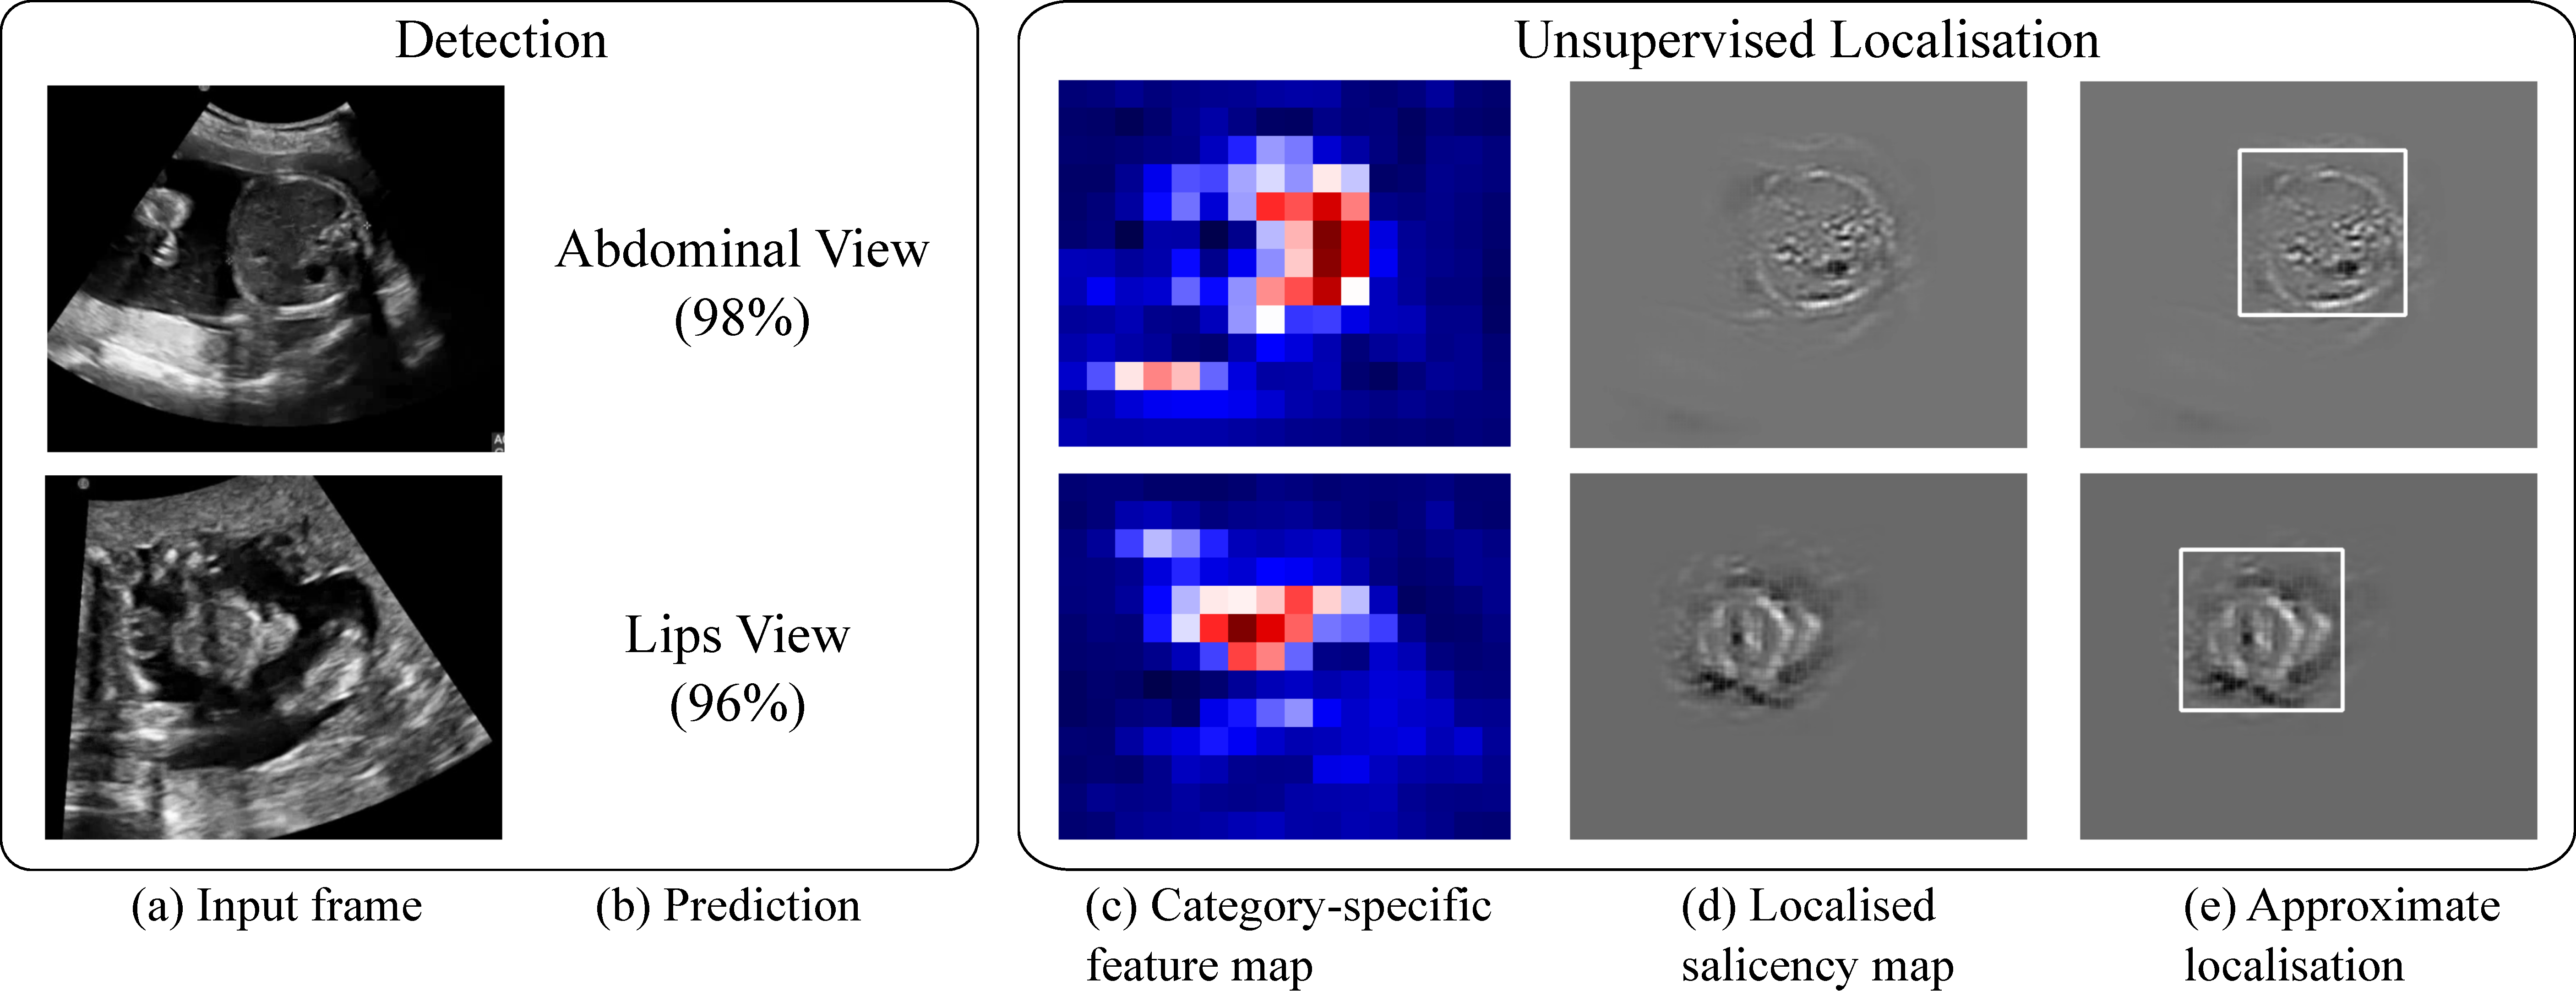
\includegraphics[width=0.99\textwidth]{overview}
\end{minipage} 
}

%%% Method %%%%%%%%%%%%%%%%%%%%%%%%%%%%%%%%%%%%%%%%%%%%%%%%%%%%%%%%%%%%%%%%%%%%
\headerbox{Method}{name=method,column=1, span=2, below=overview, bottomaligned=motivation}{

We employed a {\bf fully convolutional} neural network (i.e. no fully connected layers):\\
\vspace{-4pt}\\
\begin{minipage}[c]{\textwidth}
    \centering
    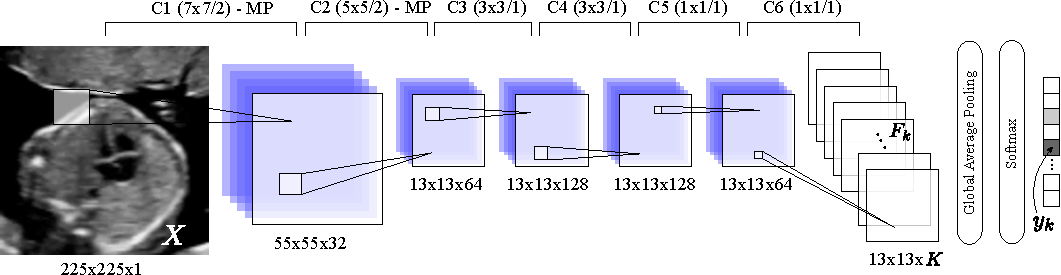
\includegraphics[width=0.95\textwidth]{convnet}
\end{minipage}\\
\vspace{1pt}\\
\emph{Training:} To enable robust detection in videos a very large background class 
of randomly sampled video frames was added. To address class imbalance (FG/BG), 
stratified mini batches were used. 
}

%%% Localisation %%%%%%%%%%%%%%%%%%%%%%%%%%%%%%%%%%%%%%%%%%%%%%%%%%%%%%%%%%%%%%%
\headerbox{Localisation}{name=localisation,column=2,span=1, below=method}{ 

After obtaining the class $k$ in the forward-pass, the saliency map can be obtained by solving:
$$S^{(i,j)}_k = \frac{\partial F_k^{(p,q)}}{\partial X^{(i,j)}}.$$
\begin{itemize}[leftmargin=1.4em]
\compresslist
  \item This is calculated using {\bf guided backpropagation}\cite{springenberg2014striving}.
  \item To achieve {\bf better localisation} we only backpropagate from 10\% most 
  active neurons in the category-specific feature map. 
\end{itemize}
\begin{minipage}[c]{\textwidth}
    \centering
    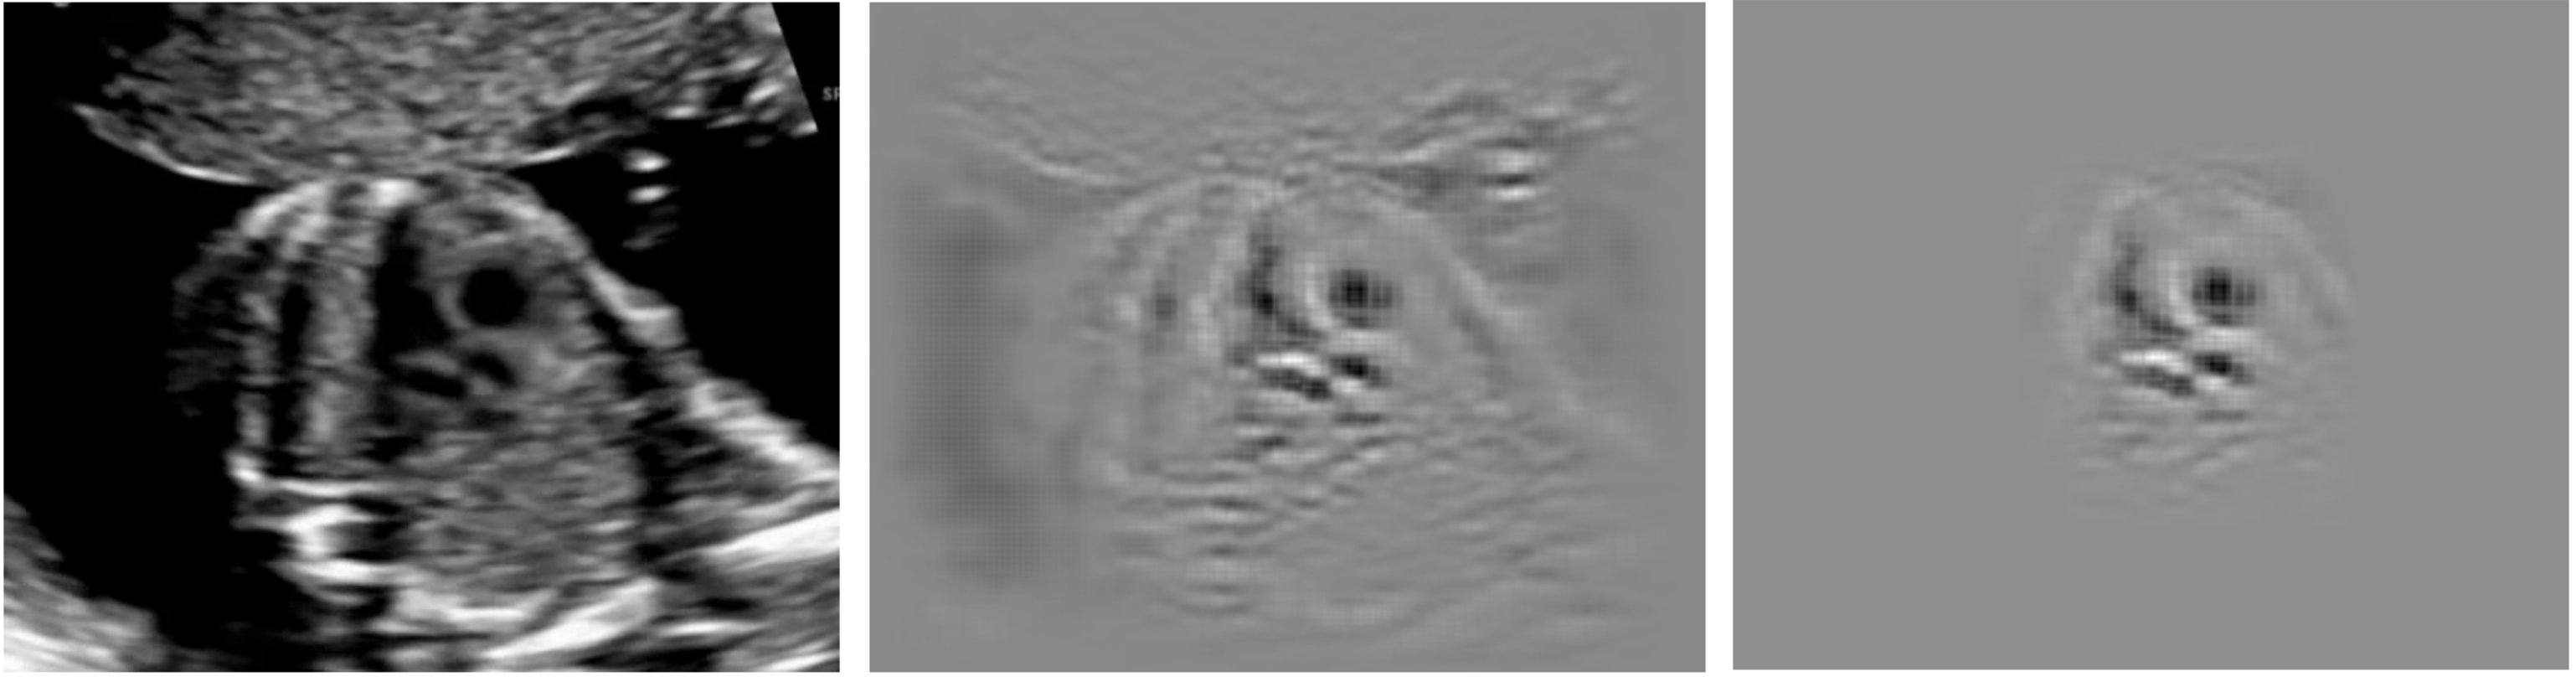
\includegraphics[width=0.99\textwidth]{lvot_saliency}
    {\scriptsize (a) input \hspace{0.9cm} (b) normal sal. \hspace{0.2cm} (c) localised sal.}
\end{minipage}
\vspace{0.3em}\\
The bounding boxes are obtained by:\vspace{3pt}
\begin{itemize}[leftmargin=1.4em]
\compresslist
   \item Blurring the absolute value $|S_k|$ using a 25x25 Gaussian kernel.
   \item Applying Otsu thresholding \cite{otsu1975threshold}.
   \item Computing the minimum bounding box of the components in the thresholded image.
\end{itemize}

}

%%% Results %%%%%%%%%%%%%%%%%%%%%%%%%%%%%%%%%%%%%%%%%%%%%%%%%%%%%%%%%%%%%%%%%%%
\headerbox{Results}{name=results,column=0,span=2, below=motivation}{

{\bf Classification results including background class:} \\

\begin{minipage}[c]{\textwidth}
   \centering
   \begin{tabular}{ l l l  | l l l | l l l }
     \toprule
     {\bf view} & {\bf $pc$} & {\bf $rc$} & {\bf view} & {\bf $pc$} & {\bf $rc$}  & {\bf view} & {\bf $pc$} & {\bf $rc$}\\
     \midrule
          Brain (Vt.)  & 0.96 & 0.90 & Lips    & 0.85 & 0.88  & LVOT & 0.63 & 0.63 \\
          Brain (Cb.)  & 0.92 & 0.94 & Profile & 0.71 & 0.82  & RVOT & 0.40 & 0.46 \\
          Abdominal    & 0.85 & 0.80 & Femur   & 0.79 & 0.93  & 3VV  & 0.46 & 0.60 \\
          Kidneys      & 0.64 & 0.87 & Spine   & 0.51 & 0.99  & 4CH  & 0.61 & 0.74 \\
          Background   & 0.96 & 0.93 &         &              &      &      &      \\
     \bottomrule
     \end{tabular}
\end{minipage}\\ 
\vspace{3pt}\\
{\bf Retrieval and localisation results from video with >30000 frames:} \\
\vspace{-2pt}\\
\begin{minipage}[c]{\textwidth}
    \centering
    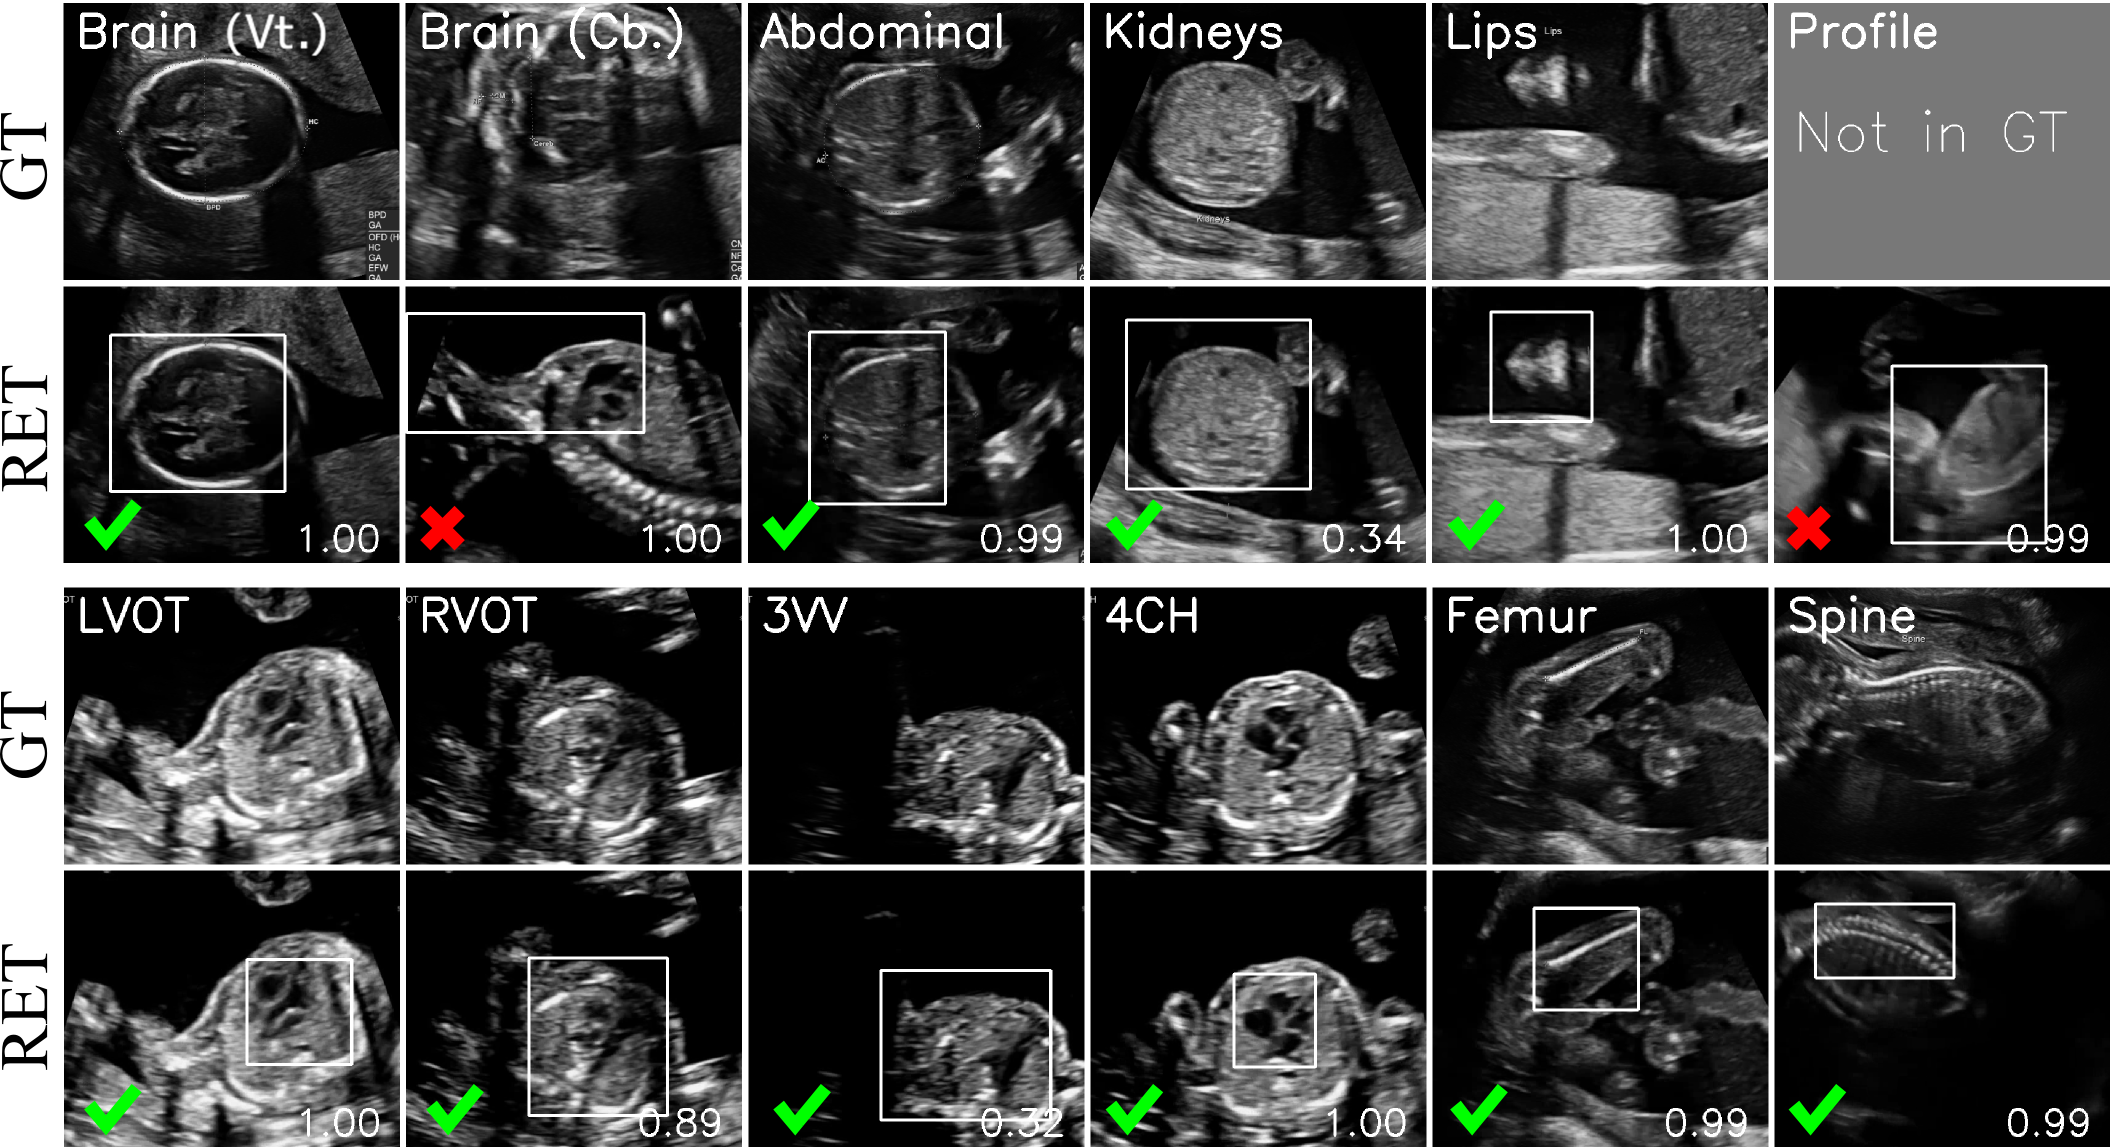
\includegraphics[width=0.90\textwidth]{ret_loc_collage_final_fixed_part2}
\end{minipage}

} 

%%% Conclusion %%%%%%%%%%%%%%%%%%%%%%%%%%%%%%%%%%%%%%%%%%%%%%%%%%%%%%%%%%%%%%%%
\headerbox{Conclusion and Future work}{name=conclusion,column=0,span=2, below=results, above=bottom}{

\begin{multicols}{2}
We present the {\bf first automatic real-time} system for standard scan plane 
detection in free-hand 2D fetal US streams.\\\vspace{-10pt}\\
\emph{Future work:} (1) Evaluate localisation with {\bf expert annotations}, 
(2) develop more principled localisation using minimal annotations, (3) use saliency 
for other tasks such as {\bf segmentation} or {\bf automatic measurements}, 
(4) improve robustness of scan plane detection across data acquired using 
different scanner models. 
\end{multicols} 

}

%%% References %%%%%%%%%%%%%%%%%%%%%%%%%%%%%%%%%%%%%%%%%%%%%%%%%%%%%%%%%%%%%%%%
\headerbox{References}{name=references,column=2, below=localisation, bottomaligned=conclusion}{ 

% make text smaller in this box
\footnotesize

% Remove the "References":
% http://tex.stackexchange.com/questions/33316/bibtex-with-no-references-title
\renewcommand\refname{}   
\vspace*{-1.5em}

\bibliographystyle{ieeetr}
\bibliography{refs}{}
}

\end{poster}
\end{document}
